%  !TeX  root  =  user_guide.tex

\chapter{Features at a Glance}\label{feature_glance}

% when the revision of a section has been finalized,
% comment out the following line:
% \updatedisclaimer

After a first and simple sample session in Section \ref{label_getstarted} we now
want to give you a more detailed overview of the features of QGIS.
Most features presented in the following chapters will be explained and described in
own sections later in the manual.

\section{Starting and Stopping QGIS}\label{label_startinqgis}

In Section \ref{samplesession} you already learned how to start QGIS. We will
repeat this here and you will see that QGIS also provides further command line options.

\begin{itemize}
\item \nix{Assuming that QGIS is installed in the PATH, you can start QGIS
by typing: \usertext{qgis}  at a command prompt or by double clicking on the QGIS
application link (or shortcut) on the desktop or in the application menu.}
\item \win{Start QGIS using the Start menu or desktop shortcut,
or double click on a QGIS project file.}
\item \osx{Double click the icon in your Applications folder. If you need to start QGIS
in a shell, run /path-to-installation-executable/Contents/MacOS/Qgis.}
\end{itemize}

To stop QGIS, click the menu options \{\nix{}\win{File} \osx{QGIS}\} \arrow Quit,
or use the shortcut \keystroke{Ctrl+Q}.

\subsection{Command Line Options}\index{command line options}
\label{label_commandline}

\nix QGIS supports a number of options when started from the command line. To
get a list of the options, enter \usertext{qgis ---help} on the command line.
The usage statement for QGIS is:

\small
\begin{verbatim}
qgis --help
Quantum GIS - 1.7.0-Wroclaw 'Wroclaw' (exported)
Quantum GIS (QGIS) is a viewer for spatial data sets, including
raster and vector data.
Usage: qgis [options] [FILES]
  options:
        [--snapshot filename]           emit snapshot of loaded datasets to given file
        [--width width]                 width of snapshot to emit
        [--height height]               height of snapshot to emit
        [--lang language]               use language for interface text
        [--project projectfile]         load the given QGIS project
        [--extent xmin,ymin,xmax,ymax]  set initial map extent
        [--nologo]                      hide splash screen
        [--noplugins]                   don't restore plugins on startup
        [--optionspath path]            use the given QSettings path
        [--configpath path]             use the given path for all user configuration
        [--help]                        this text

  FILES:
    Files specified on the command line can include rasters,
    vectors, and QGIS project files (.qgs):
     1. Rasters - Supported formats include GeoTiff, DEM
        and others supported by GDAL
     2. Vectors - Supported formats include ESRI Shapefiles
        and others supported by OGR and PostgreSQL layers using
        the PostGIS extension
\end{verbatim}
\normalsize

\begin{Tip} \caption{\textsc{Example Using command line arguments}}
You can start QGIS by specifying one or more data files
on the command line. For example, assuming you are in the
qgis\_sample\_data directory, you could start QGIS with a vector layer
and a raster file set to load on startup using the following command:
\usertext{qgis ./raster/landcover.img ./gml/lakes.gml}
\end{Tip}

\minisec{Command line option \usertext{---snapshot}}
This option allows you to create a snapshot in PNG format from the current view.
This comes in handy when you have a lot of projects and want to
generate snapshots from your data.

Currently it generates a PNG-file with 800x600 pixels. This can be adapted
using the \usertext{---width} and \usertext{---height} command line
arguments. A filename can be added after \usertext{---snapshot}.

\minisec{Command line option \usertext{---lang}}
Based on your locale QGIS, selects the correct localization. If you would like
to change your language, you can specify a language code. For example:
\usertext{---lang=it}
starts QGIS in italian localization. A list of currently supported
languages with language code and status is provided at
\url{http://www.qgis.org/wiki/GUI_Translation_Progress}

\minisec{Command line option \usertext{---project}}
Starting QGIS with an existing project file is also possible. Just
add the command line option \usertext{---project} followed by your project
name and QGIS will open with all layers loaded described in the given file.

\minisec{Command line option \usertext{---extent}}
To start with a specific map extent use this option. You need to add the bounding box of your extent in the following order separated by a comma:
\begin{verbatim}
--extent xmin,ymin,xmax,ymax
\end{verbatim}

\minisec{Command line option \usertext{---nologo}}
This command line argument hides the splash screen when you start QGIS.

\minisec{Command line option \usertext{---noplugins}}
If you have trouble at startup with plugins, you can avoid loading them at startup. They will still be available in Plugins Manager afterwards.

\minisec{Command line option \usertext{---optionspath}}
You can have multiple configurations and decide which one to use when starting QGIS using this option. See \ref{subsec:gui_options} to check where does the operating system save the settings files. Presently there is no way to specify in which file where to write the settings, therefore you can create a copy of the original settings file and rename it.

\minisec{Command line option \usertext{---configpath}}
This option is similar to the one above, but furthermore overrides the default path (~/.qgis) for user configuration and forces QSettings to use this directory, too. This allows users to e.g. carry QGIS installation on a flash drive together with all plugins and settings
 
\section{QGIS GUI}\index{main window}
\label{label_qgismainwindow}

When QGIS starts, you are presented with the GUI as shown below
(the numbers 1 through 6 in yellow ovals refer to the six major areas of the
interface as discussed below):

\begin{figure}[ht]
   \centering
    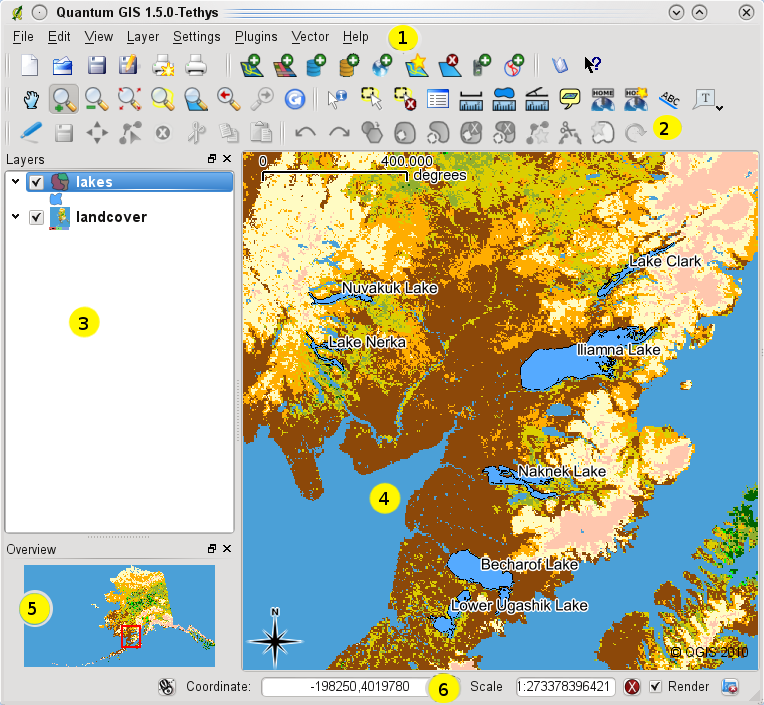
\includegraphics[clip=true, width=12cm]{startup}
    \caption{QGIS GUI with Alaska sample data \nixcaption (KDE)} \label{fig:startup}
\end{figure}

\textbf{Note:} Your window decorations (title bar, etc.) may appear
different depending on your operating system and window manager.\\

The QGIS GUI is divided into six areas:

\begin{tabular}{p{5cm} p{5cm}}
%\centering
1. Menu Bar & 4. Map View \\
2. Tool Bar & 5. Map Overview \\
3. Map Legend & 6. Status Bar \\
\end{tabular}

These six components of the QGIS interface are described in more detail in
the following sections. Two more sections present keyboard shortcuts and
context help.

% \newpage

\subsection{Menu Bar}\label{label_menubar}
\index{menus}

The menu bar provides access to various QGIS features using a standard
hierarchical menu. The top-level menus and a summary of some of the
menu options are listed below, together with the icons of the corresponding
tools as they appear on the toolbar, as well as keyboard
shortcuts.\footnote{Keyboard shortcuts can now be configured manually
(shortcuts presented in this section are the defaults), using the Configure
Shortcuts tool under Settings Menu.}
Although most menu options have a corresponding tool and vice-versa,
the menus are not organized quite like the toolbars.
The toolbar containing the tool is listed after each menu option as a checkbox
entry. For more information about tools and toolbars, see Section
\ref{label_toolbars}.

\begin{tabbing}
\hspace{5.5cm}\=\hspace{3cm}\=\hspace{3.5cm}\= \kill
\hspace{1cm} Menu Option \> Shortcut \> Reference \> Toolbar\\
\end{tabbing}

\begin{itemize}
\item \mainmenuopt{File}
\begin{tabbing}
\hspace{4.5cm}\=\hspace{3cm}\=\hspace{3.5cm}\= \kill
\dropmenuopttwo{mActionFileNew}{New Project}
	\> \keystroke{Ctrl+N}
	\> see Section \ref{sec:projects}
	\> \dropmenucheck{File} \\
\dropmenuopttwo{mActionFileOpen}{Open Project}
	\> \keystroke{Ctrl+O}
	\> see Section \ref{sec:projects}
	\> \dropmenucheck{File} \\
\dropmenuopt{Open Recent Projects}
	\>
	\> see Section \ref{sec:projects} \\
\dropmenuopttwo{mActionFileSave}{Save Project}
	\> \keystroke{Ctrl+S}
	\> see Section \ref{sec:projects}
	\> \dropmenucheck{File} \\
\dropmenuopttwo{mActionFileSaveAs}{Save Project As}
	\> \keystroke{Ctrl+Shift+S}
  \> see Section \ref{sec:projects}
	\> \dropmenucheck{File} \\
\dropmenuopttwo{mActionSaveMapAsImage}{Save as Image}
	\>
	\> see Section \ref{sec:output} \\
\dropmenuopttwo{mActionNewComposer}{New Print Composer}
        \> \keystroke{Ctrl+P}
        \> see Section \ref{label_printcomposer}
        \> \dropmenucheck{File} \\
\dropmenuopttwo{mActionComposerManager}{Composer manager}
	\>
	\> see Section \ref{label_printcomposer}
	\> \dropmenucheck{File} \\
\dropmenuopt{Print Composers}
	\>
	\> see Section \ref{label_printcomposer} \\
\dropmenuopttwo{mActionFileExit}{Exit}
	\> \keystroke{Ctrl+Q} \\
\end{tabbing}

\item \mainmenuopt{Edit}
\begin{tabbing}
\hspace{4.5cm}\=\hspace{3cm}\=\hspace{3.5cm}\= \kill
\dropmenuopttwo{mActionUndo}{Undo}
        \> \keystroke{Ctrl+Z}
        \> see Section \ref{sec:advanced_edit}
        \> \dropmenucheck{Advanced Digitizing} \\
\dropmenuopttwo{mActionRedo}{Redo}
        \> \keystroke{Ctrl+Shift+Z}
        \> see Section \ref{sec:advanced_edit}
        \> \dropmenucheck{Advanced Digitizing} \\
\dropmenuopttwo{mActionEditCut}{Cut Features}
	\> \keystroke{Ctrl+X}
	\> see Section \ref{sec:edit_existing_layer}
	\> \dropmenucheck{Digitizing} \\
\dropmenuopttwo{mActionEditCopy}{Copy Features}
	\> \keystroke{Ctrl+C}
	\> see Section \ref{sec:edit_existing_layer}
	\> \dropmenucheck{Digitizing} \\
\dropmenuopttwo{mActionEditPaste}{Paste Features}
	\> \keystroke{Ctrl+V}
	\> see Section \ref{sec:edit_existing_layer}
	\> \dropmenucheck{Digitizing} \\
\dropmenuopttwo{mActionEditPaste}{Move Feature}
        \>
        \> see Section \ref{sec:edit_existing_layer}
        \> \dropmenucheck{Digitizing} \\
\dropmenuopttwo{mActionDeleteSelected}{Delete Selected}
        \>
        \> see Section \ref{sec:edit_existing_layer}
        \> \dropmenucheck{Digitizing} \\
\dropmenuopttwo{mActionSimplify}{Simplify Feature}
        \>
        \> see Section \ref{sec:advanced_edit}
        \> \dropmenucheck{Advanced Digitizing} \\
\dropmenuopttwo{mActionAddRing}{Add Ring}
        \>
        \> see Section \ref{sec:advanced_edit}
        \> \dropmenucheck{Advanced Digitizing} \\
\dropmenuopttwo{mActionAddIsland}{Add Part}
        \>
        \> see Section \ref{sec:advanced_edit}
        \> \dropmenucheck{Advanced Digitizing} \\
\dropmenuopttwo{mActionDeleteRing}{Delete Ring}
        \>
        \> see Section \ref{sec:advanced_edit}
        \> \dropmenucheck{Advanced Digitizing} \\
\dropmenuopttwo{mActionDeletePart}{Delete Part}
        \>
        \> see Section \ref{sec:advanced_edit}
        \> \dropmenucheck{Advanced Digitizing} \\
\dropmenuopttwo{mActionReshape}{Reshape Features}
        \>
        \> see Section \ref{sec:advanced_edit}
        \> \dropmenucheck{Advanced Digitizing} \\
\dropmenuopttwo{mActionSplitFeatures}{Split Features}
        \>
        \> see Section \ref{sec:advanced_edit}
        \> \dropmenucheck{Advanced Digitizing} \\
\dropmenuopttwo{mActionMergeFeatures}{Merge selected Features}
        \>
        \> see Section \ref{sec:advanced_edit}
        \> \dropmenucheck{Advanced Digitizing} \\
\dropmenuopttwo{mActionMergeFeatures}{Merge attributes of selected Features}
        \>
        \> see Section \ref{sec:advanced_edit}
        \> \dropmenucheck{Advanced Digitizing} \\
\dropmenuopttwo{mActionNodeTool}{Node Tool}
        \>
        \> see Section \ref{sec:edit_existing_layer}
        \> \dropmenucheck{Digitizing} \\
\dropmenuopttwo{mActionRotatePointSymbols}{Rotate Point Symbols}
        \>
        \> see Section \ref{sec:advanced_edit}
        \> \dropmenucheck{Advanced Digitizing} \\
\end{tabbing}

After activating \toolbtntwo{mActionToggleEditing}{Toggle editing} mode
for a layer, you will find a capture feature icon in the \mainmenuopt{Edit}
menu depending on the layer type (point, line or polygon). \\

\begin{tabbing}
\hspace{4.5cm}\=\hspace{3cm}\=\hspace{3.5cm}\= \kill
\dropmenuopttwo{mActionCapturePoint}{Capture Point}
        \>
        \> see Section \ref{sec:edit_existing_layer}
        \> \dropmenucheck{Digitizing} \\
\dropmenuopttwo{mActionCaptureLine}{Capture Line}
        \>
        \> see Section \ref{sec:edit_existing_layer}
        \> \dropmenucheck{Digitizing} \\
\dropmenuopttwo{mActionCapturePolygon}{Capture Polygon}
        \>
        \> see Section \ref{sec:edit_existing_layer}
        \> \dropmenucheck{Digitizing} \\
\end{tabbing}


\item \mainmenuopt{View}
\begin{tabbing}
\hspace{4.5cm}\=\hspace{3cm}\=\hspace{3.5cm}\= \kill
\dropmenuopttwo{mActionPan}{Pan Map}
	\>
	\> \> \dropmenucheck{Map Navigation} \\
\dropmenuopttwo{mActionZoomIn}{Zoom In}
	\> \keystroke{Ctrl++}
	\> \> \dropmenucheck{Map Navigation} \\
\dropmenuopttwo{mActionZoomOut}{Zoom Out}
	\> \keystroke{Ctrl+-}
	\> \> \dropmenucheck{Map Navigation} \\
\dropmenuopt{Select}
	\> 
	\> see Section \ref{sec:selection} 
	\> \dropmenucheck{Attributes} \\
\dropmenuopttwo{mActionIdentify}{Identify Features}
	\> \keystroke{Ctrl-Shift-I}
	\> \> \dropmenucheck{Attributes} \\
\dropmenuopt{Measure}
	\> 
	\> see Section \ref{sec:measure}
	\> \dropmenucheck{Attributes} \\
\dropmenuopttwo{mActionOpenTable}{Zoom Full}
	\> \keystroke{Ctrl-Shift-F}
	\> \> \dropmenucheck{Map Navigation} \\
\dropmenuopttwo{mActionZoomToLayer}{Zoom To Layer}
	\>
	\> \> \dropmenucheck{Map Navigation} \\
\dropmenuopttwo{mActionZoomToSelected}{Zoom To Selection}
	\> \keystroke{Ctrl+J}
	\> \> \dropmenucheck{Map Navigation} \\
\dropmenuopttwo{mActionZoomLast}{Zoom Last}
	\>
	\> \> \dropmenucheck{Map Navigation} \\
\dropmenuopttwo{mActionZoomNext}{Zoom Next}
	\>
	\> \> \dropmenucheck{Map Navigation} \\
\mainmenuopt{Zoom Actual Size}
	\>
	\> \>  \\
\dropmenuopttwo{mActionMapTips}{Map Tips}
	\>
	\> \> \dropmenucheck{Attributes} \\
\dropmenuopttwo{mActionNewBookmark}{New Bookmark}
	\> \keystroke{Ctrl+B}
	\> see Section \ref{sec:bookmarks}
\> \dropmenucheck{Attributes} \\
\dropmenuopttwo{mActionShowBookmarks}{Show Bookmarks}
	\> \keystroke{Ctrl-Shift-B}
	\> see Section \ref{sec:bookmarks}
	\> \dropmenucheck{Attributes} \\
\dropmenuopttwo{mActionDraw}{Refresh}
	\> \keystroke{Ctrl+R}
	\> \> \dropmenucheck{Map Navigation} \\
\mainmenuopt{Tile scale slider}
	\>
	\> see Section \ref{sec:tilesets}
	\> \dropmenucheck{Tile scale} \\
\mainmenuopt{Live GPS tracking}
	\>
	\> see Section \ref{sec:gpstracking}
	\> \dropmenucheck{GPS Information} \\
\end{tabbing}

\item \mainmenuopt{Layer}
\begin{tabbing}
\hspace{5cm}\=\hspace{3cm}\=\hspace{3.5cm}\= \kill
\dropmenuopt{New}
	\>
	\> see Section \ref{sec:create shape}
	\> \dropmenucheck{Manage Layers} \\
\dropmenuopttwo{mActionAddNonDbLayer}{Add Vector Layer}
	\> \keystroke{Ctrl+Shift+V}
	\>
	see Section \ref{label_workingvector}
	\> \dropmenucheck{Manage Layers} \\
\dropmenuopttwo{mActionAddRasterLayer}{Add Raster Layer}
	\> \keystroke{Ctrl+Shift+R}
	\>
	see Section \ref{label_raster}
	\> \dropmenucheck{Manage Layers} \\
\dropmenuopttwo{mActionAddLayer}{Add PostGIS Layer}
	\> \keystroke{Ctrl+Shift+D}
	\>
	see Section \ref{label_postgis}
        \> \dropmenucheck{Manage Layers} \\
\dropmenuopttwo{mActionAddSpatiaLiteLayer}{Add SpatiaLite Layer}
        \> \keystroke{Ctrl+Shift+L}
        \>
        see Section \ref{label_spatialite}
	\> \dropmenucheck{Manage Layers} \\
\dropmenuopttwo{mActionAddWmsLayer}{Add WMS Layer}
	\> \keystroke{Ctrl+Shift+W}
	\>
	see Section \ref{sec:ogc-wms}
	\> \dropmenucheck{Manage Layers} \\
\dropmenuopttwo{mActionOpenTable}{Open Attribute Table}
	\> \>
	\> \dropmenucheck{Attributes} \\
\dropmenuopttwo{mActionFileSave}{Save edits}
        \> \>
        \> \dropmenucheck{Digitizing} \\
\dropmenuopttwo{mActionToggleEditing}{Toggle editing}
	\> \>
	\> \dropmenucheck{Digitizing} \\
\mainmenuopt{Save as...}
	\\
\mainmenuopt{Save selection as vector file...}
	\> 
	\> See \ref{sec:attribute table}
	\> \\
\dropmenuopttwo{mActionRemoveLayer}{Remove Layer}
	\> \keystroke{Ctrl+D}
	\>
	\> \\
\mainmenuopt{Set CRS of Layer(s)}
	\> \keystroke{Ctrl+Shift+C}
	\>
	\> \\
\mainmenuopt{Set project CRS from Layer}
	\\
\mainmenuopt{Properties}
	\\
\mainmenuopt{Query...}
	\\
\dropmenuopttwo{labeling}{Labeling}
	\>
	\>
	\\
\dropmenuopttwo{mActionInOverview}{Add to Overview}
	\> \keystroke{Ctrl+Shift+O}
	\>
	\> 
\dropmenucheck{Manage Layers} 
	\\
\dropmenuopttwo{mActionAddAllToOverview}{Add All To Overview}
	\>
	\>
	\\
\dropmenuopttwo{mActionRemoveAllFromOverview}{Remove All From Overview}
	\>
	\>
	\\
\dropmenuopttwo{mActionShowAllLayers}{Show All Layers}
	\> \keystroke{Ctrl+Shift+U}
	\>
	\> \dropmenucheck{Manage Layers} \\
\dropmenuopttwo{mActionHideAllLayers}{Hide All Layers}
	\> \keystroke{Ctrl+Shift+H}
	\>
	\> \dropmenucheck{Manage Layers} \\
\end{tabbing}

\item \mainmenuopt{Settings}
\begin{tabbing}
\hspace{5cm}\=\hspace{3cm}\=\hspace{3.5cm}\= \kill
\dropmenuopt{Panels}
	\>
	\>
	\\
\dropmenuopt{Toolbars}
	\>
	\>
	\\
\mainmenuopt{Toggle Full Screen Mode}
	\>\keystroke{Ctrl-F}
	\>
	\\
\dropmenuopttwo{mActionProjectProperties}{Project Properties}
	\> \keystroke{Ctrl-Shift-P}
	\> see Section \ref{sec:projects} \\
\dropmenuopttwo{mActionCustomProjection}{Custom CRS}
        \> \> see Section \ref{sec:customprojections} \\
\mainmenuopt{Style Manager}
        \> \> \\
\dropmenuopttwo{mActionOptions}{Configure shortcuts}
        \> \> \\
\dropmenuopttwo{mActionOptions}{Options}
        \> \> see Section \ref{subsec:gui_options} \\
\dropmenuopt{Snapping Options}
	\>
	\>
	\\
\end{tabbing}

\item \mainmenuopt{Plugins} - (Futher menu items are added by plugins as they are loaded.)
\begin{tabbing}
\hspace{5cm}\=\hspace{3cm}\=\hspace{3.5cm}\= \kill
\dropmenuopttwo{mActionShowPluginManager}{Manage Plugins}
	\> \> see Section \ref{sec:managing_plugins} \dropmenucheck{Plugins}
	\\
	\mainmenuopt{Python Console}
        \> \>
        \\
\end{tabbing}

\item \mainmenuopt{Raster}
\begin{tabbing}
\hspace{5cm}\=\hspace{3cm}\=\hspace{3.5cm}\= \kill
\mainmenuopt{Raster calculator}
        \>
        \> see Section \ref{sec:raster_calc}
        \>  \\
\end{tabbing}

\item \mainmenuopt{Help}
\begin{tabbing}
\hspace{5cm}\=\hspace{3cm}\=\hspace{3.5cm}\= \kill
\dropmenuopttwo{mActionHelpContents}{Help Contents}
	\> \keystroke{F1}
	\>
	\> \dropmenucheck{Help}\\
\mainmenuopt{API Documentation}
        \>
        \> 
        \>  \\
\dropmenuopttwo{mActionQgisHomePage}{QGIS Home Page}
	\> \keystroke{Ctrl+H}
	\>
	\\
\dropmenuopttwo{mActionCheckQgisVersion}{Check QGIS Version}
	\\
\dropmenuopttwo{mActionHelpAbout}{About}
	\\
\dropmenuopttwo{mActionHelpSponsors}{QGIS Sponsors}
	\\
\end{tabbing}

\end{itemize}

\textbf{Note:} \nix The Menu Bar items listed above are the default ones in KDE window
manager. In GNOME, Settings menu is missing and its items are to be found
there:
\begin{tabbing}
\dropmenuopttwo{mActionProjectProperties}{Project Properties} \hspace{3cm}\=
\dropmenucheck{File menu} \\
\dropmenuopttwo{mActionOptions}{Options} \hspace{3cm}\>
\dropmenucheck{Edit}\\
\dropmenuopttwo{mActionOptions}{Configure Shortcuts} \hspace{3cm}\>
\dropmenucheck{Edit}\\
\mainmenuopt{Style Manager} \hspace{3cm}\>
\dropmenucheck{Edit}\\
\dropmenuopttwo{mActionCustomProjection}{Custom CRS}\hspace{3cm}\>
\dropmenucheck{Edit} \\
\dropmenuopt{Panels} \hspace{3cm}\>
\dropmenucheck{View} \\
\dropmenuopt{Toolbars}   \hspace{3cm}\>
\dropmenucheck{View} \\
\mainmenuopt{Toggle Full Screen Mode} \hspace{3cm}\>
\dropmenucheck{View} \\
\mainmenuopt{Tile scale slider} \hspace{3cm}\>
\dropmenucheck{View} \\
\mainmenuopt{Live GPS tracking} \hspace{3cm}\>
\dropmenucheck{View} \\
\end{tabbing}

%See Appendix \ref{app_menu} for complete descriptions of the menu items.

\subsection{Toolbars}\label{label_toolbars}
\index{toolbars}

The toolbars provide access to most of the same functions as the menus,
plus additional tools for interacting with the map. Each toolbar item has
popup help available. Hold your mouse over the item and a short description of
the tool's purpose will be displayed.

Every menubar can be moved around according to your needs. Additionally every
menubar can be switched off using your right mouse button context menu holding
the mouse over the toolbars.

\begin{Tip}
\caption{\textsc{Restoring toolbars}} \index{layout!toolbars}
If you have accidentally hidden all your toolbars, you can get them
back by choosing menu option \mainmenuopt{Settings} \arrow \dropmenuopt{Toolbars}.
\end{Tip}

\subsection{Map Legend}\label{label_legend}
\index{legend}

The map legend area lists all the layers in the project.
The checkbox in each legend entry can be used to show or hide the layer.\index{layer!visibility}
A layer can be selected and dragged up or down in the legend to change the
z-ordering. Z-ordering means that layers listed nearer the top of the legend are
drawn over layers listed lower down in the legend.

Layers in the legend window can be organised into groups. To do so, right click
in the legend window and choose \dropmenuopt{Add group}. Type in a name for the
group and press \keystroke{Enter}. Now click on an existing layer and drag it
onto the group. Also, if new layers are added to the project while a group is
selected, they will automatically be placed in the group.
To bring a layer out of a group you can drag it out, or right click on it and 
choose \dropmenuopt{Make to toplevel item}.
Groups can be nested inside other groups.
The checkbox for a group will show or hide all the layers in the group
with one click.

The content of the right mouse button context menu depends on whether the selected legend item
is a raster or a vector layer. For GRASS vector layers \dropmenuopt{toggle editing} is not
available. See section \ref{grass_digitising} for information on editing GRASS vector layers.

\begin{itemize}

\item \textbf{Right mouse button menu for raster layers}
\begin{itemize}
\item \dropmenuopt{Zoom to layer extent}
\item \dropmenuopt{Zoom to best scale (100\%)}
\item \dropmenuopt{Show in overview}
\item \dropmenuopt{Remove}
\item \dropmenuopt{Properties}
\item \dropmenuopt{Rename}
\item \dropmenuopt{Add Group}
\item \dropmenuopt{Expand all}
\item \dropmenuopt{Collapse all}
%%\item \dropmenuopt{Show file groups}
\end{itemize}

\item \textbf{Right mouse button menu for vector layers}
\begin{itemize}
\item \dropmenuopt{Zoom to layer extent}
\item \dropmenuopt{Show in overview}
\item \dropmenuopt{Remove}
\item \dropmenuopt{Open attribute table}
\item \dropmenuopt{Toggle editing (not available for GRASS layers)}
\item \dropmenuopt{Save as}
\item \dropmenuopt{Save selection as}
\item \dropmenuopt{Query}
\item \dropmenuopt{Properties}
%% \item \dropmenuopt{Make to toplevel item}
\item \dropmenuopt{Rename}
\item \dropmenuopt{Add Group}
\item \dropmenuopt{Expand all}
\item \dropmenuopt{Collapse all}
%%\item \dropmenuopt{Show file groups}
\end{itemize}

\item \textbf{Right mouse button menu for layer groups}
\begin{itemize}
\item \dropmenuopt{Zoom to group}
\item \dropmenuopt{Remove}
\item \dropmenuopt{Set group CRS}
\item \dropmenuopt{Rename}
\item \dropmenuopt{Add Group}
\item \dropmenuopt{Expand all}
\item \dropmenuopt{Collapse all}
%%\item \dropmenuopt{Show file groups}
\end{itemize}

\end{itemize}

It is possible to select more than one Layer or Group at the same time 
by holding down the \keystroke{CTRL}-Key while selecting the Layers with the 
left mouse button. You can than move all selected Layers to a new Group at 
the same time.

You are also able to delete more than one Layer or Group at once by selecting 
several Layers with the \keystroke{CTRL}-Key and pressing \keystroke{CTRL-D} afterwards.
This way all selected Layers or Groups will be removed from the Layerlist.

%% isn't included in Titan anymore, except for an "toggle overview"
%Each legend entry can show the following mini icons:
%
%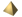
\includegraphics[width=0.7cm]{pyramid} This is a raster
%that has pyramids built for it to improve rendering efficiency (see
%Section \ref{raster_pyramids}).\\
%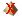
\includegraphics[width=0.7cm]{no_pyramid} This is a
%raster that has no pyramid layers (see Section \ref{raster_pyramids}).\\
%
\includegraphics[width=0.7cm]{inoverview} This layer is
%shown in the overview map area as well as in the main map window.\\
%
\includegraphics[width=0.7cm]{editable} This is a vector
%layer that is currently enabled for editing.\\

\subsection{Map View}\label{label_mapview}
\index{map!view}

This is the 'business end' of QGIS - maps are displayed in this area! The
map displayed in this window will depend on the vector and raster layers you
have chosen to load (see sections that follow for more information on how to
load layers). The map view can be panned (shifting the focus of the map display
to another region) and zoomed in and out. Various other operations can be
performed on the map as described in the toolbar description above.  The map
view and the legend are tightly bound to each other - the maps in view reflect
changes you make in the legend area.

\begin{Tip}\caption{\textsc{Zooming the Map with the Mouse
Wheel}}\index{zoom!mouse wheel}
You can use the mouse wheel to zoom in and out on the map. Place
the mouse cursor inside the map area and roll the wheel forward (away from you) to
zoom in and backwards (towards you) to zoom out. The mouse cursor position is the
center where the zoom occurs. You can customize the behavior of the mouse
wheel zoom using the \tab{Map tools} tab under the \mainmenuopt{Settings} \arrow
\dropmenuopt{Options} menu.
\end{Tip}

\begin{Tip}\caption{\textsc{Panning the Map with the Arrow Keys and Space
Bar}}\index{pan!arrow keys}
You can use the arrow keys to pan in the map. Place the mouse cursor
inside the map area and click on the right arrow key to pan East, left arrow
key to pan West, up arrow key to pan North and down arrow key to pan South.
You can also pan the map using the space bar: just move the mouse while
holding down space bar.
\end{Tip}

\subsection{Map Overview}\label{label_mapoverview}
\index{map!overview}

The map overview panel provides a full extent view of layers added to it. It
can be selected under the menu \mainmenuopt{Settings} \arrow \dropmenuopt{Panels}.
Within the view is a rectangle showing the current map extent. This allows
you to quickly determine which area of the map you are currently viewing. Note
that labels are not rendered to the map overview even if the layers in the
map overview have been set up for labeling.

You can add a single layer to the overview by right-clicking on it in the
legend and select \checkbox{Show in overview}. You can also add layers to,
or remove all layers from the overview using the Overview tools on the toolbar.

If you click and drag the red rectangle in the overview that shows your
current extent, the main map view will update accordingly.

\subsection{Status Bar}\label{label_statusbar}

The status bar shows you your current position in map coordinates (e.g.
meters or decimal degrees) as the mouse pointer is moved across the map view.
To the left of the coordinate display in the status bar is a small button that
will toggle between showing coordinate position or the view extents of the
map view as you pan and zoom in and out.

A progress bar in the status bar shows progress of rendering
as each layer is drawn to the map view. In some cases, such as the gathering
of statistics in raster layers, the progress bar will be used to show the
status of lengthy operations.

If a new plugin or a plugin update is available, you will see a message in the
status bar. On the right side of the status bar is a small
checkbox which can be used to temporarily prevent layers being rendered to the
map view (see Section \ref{subsec:redraw_events} below). The icon 

\includegraphics[width=0.4cm]{mIconStopRendering} immediately stops the 
current map rendering process. 

At the far right of the status bar you find the EPSG code of the current 
project CRS and a projector icon. Clicking on this opens the projection properties 
for the current project.

\begin{Tip}\caption{\textsc{Calculating the correct Scale of your Map Canvas}}\index{scale!calculate}
When you start QGIS, degrees is the default unit, and it tells QGIS
that any coordinate in your layer is in degrees. To get correct scale values,
you can either change this to meter manually in the \tab{General} tab under
\mainmenuopt{Settings} \arrow \dropmenuopt{Project Properties} or you can select a project
Coordinate Reference System (CRS) clicking on the
\toolbtntwo{mIconProjectionDisabled}{CRS status}
icon in the lower right-hand corner of the statusbar. In the last case, the
units are set to what the project projection specifies, e.g. '+units=m'.
\end{Tip}

\subsection{Keyboard shortcuts}\label{shortcuts}
\index{Keyboard shortcuts}

QGIS provides default keyboard shortcuts for many features. You find them in
Section \ref{label_menubar} below. Additionally the menu option \mainmenuopt{Settings} \arrow
\dropmenuopt{Configure Shortcuts} allows to change the default keyboard
shortcuts and to add new keyboard shortcuts to QGIS features.

\begin{figure}[ht]
   \centering
   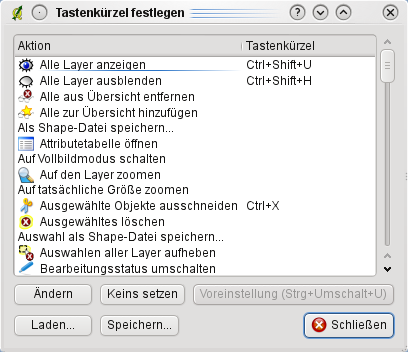
\includegraphics[clip=true, width=8cm]{shortcuts}
   \caption{Define shortcut options \nixcaption (KDE)} \label{fig:shortcuts}
\end{figure}

Configuration is very simple. Just select a feature from the list and click
on \button{Change}, \button{Set none} or \button{Set default}. Once you have
found your configuration, you can save it as XML file and load it to another
QGIS installation.

\subsection{Context help}\label{context_help}
\index{Context help}

When you need help on specific topic, you can access context help via the Help
button available in most dialogs - please note that third-party plugins can point to
dedicated web pages.

\section{Rendering}\label{subsec:redraw_events}\index{rendering}

By default, QGIS renders all visible layers whenever the map canvas must be
refreshed. The events that trigger a refresh of the map canvas include:

\begin{itemize}
\item Adding a layer
\item Panning or zooming
\item Resizing the QGIS window
\item Changing the visibility of a layer or layers
\end{itemize}

QGIS allows you to control the rendering process in a number of ways.

\subsection{Scale Dependent Rendering}\index{rendering!scale dependent}
\label{label_scaledepend}

Scale dependent rendering allows you to specify the minimum and maximum
scales at which a layer will be visible.  To set scale dependency rendering,
open the \dialog{Properties} dialog by double-clicking on the layer in the
legend. On the \tab{General} tab, set the minimum and maximum scale values and then
click on the \checkbox{Use scale dependent rendering} checkbox.

You can determine the scale values by first zooming to the level you want
to use and noting the scale value in the QGIS status bar.\index{scale}

\subsection{Controlling Map Rendering}\label{label_controlmap}

Map rendering can be controlled in the following ways:

\minisec{a) Suspending Rendering}\index{rendering!suspending}
\label{label_suspendrender}

To suspend rendering, click the \checkbox{Render} checkbox in the lower right
corner of the statusbar. When the \checkbox{Render} box is not checked, QGIS
does not redraw the canvas in response to any of the events described in
Section \ref{subsec:redraw_events}. Examples of when you might want to suspend
rendering include:

\begin{itemize}
\item Add many layers and symbolize them prior to drawing
\item Add one or more large layers and set scale dependency before drawing
\item Add one or more large layers and zoom to a specific view before drawing
\item Any combination of the above
\end{itemize}

Checking the \checkbox{Render} box enables rendering and causes and immediate
refresh of the map canvas.

\minisec{b) Setting Layer Add Option}\label{label_settinglayer}
\index{rendering!options}\index{layers!initial visibility}

You can set an option to always load new layers without drawing them. This
means the layer will be added to the map, but its visibility checkbox in the
legend will be unchecked by default. To set this option, choose
menu option \mainmenuopt{Settings} \arrow \dropmenuopt{Options} and click on the
\tab{Rendering} tab. Uncheck the \\
\checkbox{By default new layers added to the map should be displayed} checkbox.
Any layer added to the map will be off (invisible) by default.

%\minisec{Stopping Rendering}\index{rendering!halting}
%\label{label_stoprender}
%
%To stop the map drawing, press the ESC key. This will halt the refresh of
%the map canvas and leave the map partially drawn. It may take a bit of time
%between pressing ESC and the time the map drawing is halted.
%
%\textbf{NOTE}: It is currently not possible to stop rendering - this was disabled
%in qt4 port because of User Interface (UI) problems and crashes.

\minisec{c) Updating the Map Display During Rendering}
\label{label_updatemap}\index{rendering!update during drawing}

You can set an option to update the map display as features are drawn. By
default, QGIS does not display any features for a layer until the entire
layer has been rendered. To update the display as features are read from the
datastore, choose menu option \mainmenuopt{Settings} \arrow \dropmenuopt{Options}
click on the \tab{Rendering} tab. Set the feature count to an
appropriate value to update the display during rendering. Setting a value of 0
disables update during drawing (this is the default). Setting a value too low
will result in poor performance as the map canvas is continually updated
during the reading of the features. A suggested value to start with is 500.

\minisec{d) Influence Rendering Quality}
\label{label_renderquality}\index{rendering!quality}

To influence the rendering quality of the map you have 3 options. Choose menu
option \mainmenuopt{Settings} \arrow \dropmenuopt{Options} click on the
\tab{Rendering} tab and select or deselect following checkboxes.

\begin{itemize}
\item \checkbox{Make lines appear less jagged at the expense of some drawing
performance}
\item \checkbox{Fix problems with incorrectly filled polygons}
\end{itemize}

\section{Measuring}\label{sec:measure}\index{measure}

Measuring works within projected coordinate systems only (e.g., UTM). If
the loaded map is defined with a geographic coordinate system
(latitude/longitude), the results from line or area measurements will be
incorrect. To fix this you need to set an appropriate map coordinate system
(See Section~\ref{label_projections}). Both measuring modules also use the
snapping settings from the digitizing module. This is useful, if you want to
measure along lines or areas in vector layers.

To select a measure tool click on 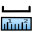
\includegraphics[width=0.7cm]{mActionMeasure} and 
select the tool you want to use.

\subsection{Measure length, areas and angles}
\index{measure:line length}
\index{measure:areas}
\index{measure:angles}

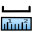
\includegraphics[width=0.7cm]{mActionMeasure}
QGIS is also able to measure real distances between given
points according to a defined ellipsoid. To configure this, choose menu option
\mainmenuopt{Settings} \arrow \dropmenuopt{Options},
click on the \tab{Map tools} tab and choose the appropriate ellipsoid. There
you can also define a rubberband color and your preferred measurement units
(meters or feet). The tool then allows you to click points on the map. Each
segment-length as well as the total shows up in the measure-window. To stop measuring click your right mouse button. \\

\includegraphics[width=0.7cm]{mActionMeasureArea} Areas can also be measured.
In the measure window the accumulated area-size appears  \\
In addition, the measuring tool will snap to the currently selected layer, provided that layer has its snapping tolerance set. (See Section~\ref{snapping_tolerance}). So if you want to measure exactly along a line feature, or around a polygon feature, first set its snapping tolerance, then select the layer. Now, when using the measuring tools, each mouse click (within the tolerance setting) will snap to that layer. \\
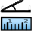
\includegraphics[width=0.7cm]{mActionMeasureAngle}
You can also measure angles, selecting Measure Angle tool. The cursor becomes
cross-shaped. Click to draw the first segment of the angle you wish to
measure, then move the the cursor to draw the desired angle. The measure
is displayed in a popup dialog.

\begin{figure}[ht]
\centering
   \subfloat[Measure lines] {\label{subfig:measure_line}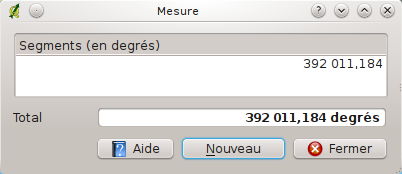
\includegraphics[clip=true, width=0.3\textwidth]{measure_line}}
     \hspace{0.33cm}
   \subfloat[Measure areas]{\label{subfig:measure_area}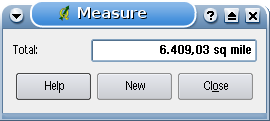
\includegraphics[clip=true, width=0.3\textwidth]{measure_area}}
     \hspace{0.33cm}
   \subfloat[Measure angles]{\label{subfig:measure_angle}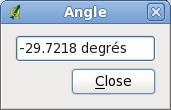
\includegraphics[clip=true, width=0.3\textwidth]{measure_angle}}
   \caption{Measure tools in action \nixcaption} \label{fig:measure}
\end{figure}

\subsection{Select and deselect features}\label{sec:selection}

The QGIS toolbar provides several tools to select features in the map canvas. 
To select one or several features just click on 

\includegraphics[width=0.7cm]{mActionSelect} and select your tool:

\begin{description}
\item 
\includegraphics[width=0.5cm]{mActionSelect} Select features
\item 
\includegraphics[width=0.5cm]{mActionSelectRectangle} Select features by rectangle
\item 
\includegraphics[width=0.5cm]{mActionSelectPolygon} Select features by polygon
\item 
\includegraphics[width=0.5cm]{mActionSelectFreehand} Select features by freehand
\item 
\includegraphics[width=0.5cm]{mActionSelectRadius} Select features by radius
\end{description} 

To deselect all selected features click on 
\includegraphics[width=0.7cm]{mActionDeselectAll}.

\section{Projects}\label{sec:projects}\index{projects}

The state of your QGIS session is considered a Project.  QGIS
works on one project at a time.  Settings are either considered
as being per-project, or as a default for new projects (see
Section \ref{subsec:gui_options}). QGIS can save the state of your
workspace into a project file using the menu options
\mainmenuopt{File} \arrow \dropmenuopttwo{mActionFileSave}{Save Project}
or \mainmenuopt{File} \arrow \dropmenuopttwo{mActionFileSaveAs}{Save Project As}.

Load saved projects into a QGIS session using
\mainmenuopt{File} \arrow \dropmenuopttwo{mActionFileOpen}{Open Project}
or \mainmenuopt{File} \arrow \\
\dropmenuopt{Open Recent Project}.

If you wish to clear your session and start fresh, choose
\mainmenuopt{File} \arrow \dropmenuopttwo{mActionFileNew}{New Project}.
Either of these menu options will prompt you to save the existing project
if changes have been made since it was opened or last saved.

The kinds of information saved in a project file include:

\begin{itemize}
\item Layers added
\item Layer properties, including symbolization
\item Projection for the map view
\item Last viewed extent
\end{itemize}

The project file is saved in XML format, so it is possible to edit
the file outside QGIS if you know what you are doing. The file format
was updated several times compared to earlier QGIS versions. Project files
from older QGIS versions may not work properly anymore. To be made aware of this,
in the \tab{General} tab under \mainmenuopt{Settings} \arrow \dropmenuopt{Options}
you can select: \\

\checkbox{Promt to save project changes when required} \\
\checkbox{Warn when opening a project file saved with an older version of QGIS}

\minisec{Project Properties}
In the properties window for the project under \nix{\mainmenuopt{File} \arrow
\dropmenuopt{Project Properties}} or \win{\mainmenuopt{Settings} \arrow
\dropmenuopt{Project Properties}} you set project specific options. These
include:

\begin{itemize}
\item In the \tab{General} tab the project title, selection and background
color, layer units, precision, and the option to save relative paths to
layers can be defined. You can define the layer units (only used when CRS 
transformation is disabled) and the precision of decimal places to use.  
\item The \tab{CRS} Coordinate Reference System tab enables you to choose the
CRS for this project, and to enable on-the-fly reprojection of raster and vector 
layers when displaying layers from a different CRS.
\item With the third \tab{Identifiable layers} tab you set (or disable) which
layers will respond to the identify tool. (See the Map tools paragraph from
the \ref{subsec:gui_options} section to enable identifying of multiple layers.)
\item The tab \tab{WMS Server} allows to define information about the QGIS 
mapserver Service Capabilities, the Extend and the CRS Restrictions. Activating 
the \checkbox{Add WKT geometry to feature info response} will allow to query the 
WMS layers.
\end{itemize}

\section{Output}\label{sec:output}
\index{output!save as image!print composer!quick print}

There are several ways to generate output from your QGIS session. We have
discussed one already in Section \ref{sec:projects}: saving as a project file.
Here is a sampling of other ways to produce output files:

\begin{itemize}
\item Menu option \dropmenuopttwo{mActionSaveMapAsImage}{Save as Image} opens
a file dialog where you select the name, path and type of image (PNG or JPG
format). A world file with extension PNGW or JPGW saved in the same folder
georeferences the image.
\item Menu option \dropmenuopttwo{mActionFilePrint}{Print Composer} opens a
dialog where you can layout and print the current map canvas (see
Section~\ref{label_printcomposer}).
\end{itemize}

\section{GUI Options}\label{subsec:gui_options}


\includegraphics[width=0.7cm,clip=true]{mActionOptions} Some basic options
for QGIS can be selected using the \dialog{Options} dialog. Select the
menu option \mainmenuopt{Settings} \arrow
\dropmenuopttwo{mActionOptions}{Options}. The tabs where you can
optmize your options are:

\minisec{General Tab}

\begin{itemize}
\item \checkbox{Promt to save project changes when required}
\item \checkbox{Warn when opening a project file saved with an older version of QGIS}
\item Change Selection and backgroud Color
\item Change the icon theme (choose between default, classic, gis and newgis)
\item Change icon size between 16, 24 and 32 pixel.
\item Define double click action in legend (choose between 'open layer properties' 
and 'open ') attribute table.
\item \checkbox{Capitalise layer names in legend}
\item \checkbox{Display classification attribute names in legend}
\item \checkbox{Create raster icons in legend}
\item \checkbox{Hide splash screen at startup}
\item \checkbox{Open identify results in a dock window (QGIS restart
required)}
\item \checkbox{Open snapping options in a dock window (QGIS restart
required)}
\item \checkbox{Open attribute table in a dock window}
\item \checkbox{Add PostGIS layers with double click and select in extended mode}
\item \checkbox{Add new layers to selected group}
\item Attribute table behavior (choose between Show all features (default), Show selected features,
show features in current canvas)
\item Define representation for NULL values
\item Add path(s) to search for additional C++ plugin libraries. 
\end{itemize}

\minisec{Rendering Tab}

\begin{itemize}
\item \checkbox{By default new layers added to the map should be displayed}
\item Define number of features to draw before updating the display.
\item \checkbox{Use render caching where possible to speed up redraws}
\item \checkbox{Make lines appear less jagged at the expense of some drawing
performance}
\item \checkbox{Fix problems with incorrectly filled polygons}
\item \checkbox{Use new generation symbology for rendering}
\item Add/remove path(s) to search for Scalable Vector Graphics (SVG) symbols
\end{itemize}

Additionally you can define wether to save the path for svg textures
absolute or relative in the \tab{General} tab of the
\mainmenuopt{Settings} \arrow \dropmenuopttwo{mActionOptions}{Project Properties}
menu.

\minisec{Map tools Tab}

\begin{itemize}
\item The Mode setting determines which layers will be shown by the Identify
tool. By switching to \usertext{Top down} or \usertext{Top down, stop at
first} instead of \usertext{Current layer} attributes for all identifiable
layers (see the Project properties section under: \ref{sec:projects} to set
which layers are identifiable) will be shown with the Identify tool.
\item \checkbox{Open feature form, if a single feature is identified}
\item Define search radius for identifying and displaying map tips as a
percentage of the map width
\item Define ellipsoid for distance calculations
\item Define rubberband color for measure tools
\item Define decimal places
\item \checkbox{Keep base unit}
\item \radiobuttonon{Define preferred measurement units (meters or feet)}
\item \radiobuttonon{Define preferred angle units (Degrees, Radians or Gon)}
\item Define Mouse wheel action (Zoom, Zoom and recenter, Zoom to mouse
cursor, Nothing)
\item Define Zoom factor for wheel mouse
\end{itemize}

\minisec{Overlays Tab}

\begin{itemize}
\item Define placement algorithm for labels (choose between central point
(standard), chain, popmusic tabu chain, popmusic tabu and popmusic chain)
\end{itemize}

\minisec{Digitizing Tab}

\begin{itemize}
\item Define Rubberband line color and line width
\item Define default snap mode (to vertex, to segment, to vertex and segment)
\item Define default snapping tolerance in map units or pixel
\item Define search radius for vertex edits in map units or pixel
\item \checkbox{Show markers only for selected features}
\item Define vertex marker style (cross (default), semi transparent circle or
none) and vertex marker size.
\item \checkbox{Reuse last entered attribute values}
\item \checkbox{Suppress attributes pop-up windows after each created feature}
\end{itemize}

\minisec{CRS Tab}

The CRS tab is devided in two areas. The first area allows to define the default 
CRS for new projects.

\begin{itemize}
\item Select a CRS and always start new projects with this CRS.
\item \checkbox{Enable on the fly reprojecion by default}
\end{itemize}

The second area allows to define the action, when a new layer is created, or when a 
layer without CRS is loaded.
\begin{itemize}
\item \radiobuttonoff{Prompt for Coordinate Reference System (CRS)}
\item \radiobuttonoff{Project wide default Coordinate Reference System (CRS) will be used}
\item \radiobuttonon{Global default Coordinate Reference System (CRS) displayed below will be used}
\end{itemize}

\minisec{Locale Tab}

\begin{itemize}
\item \checkbox{Overwrite system locale and use defined locale instead}
\item Information about active system locale
\end{itemize}

\minisec{Proxy Tab}

\begin{itemize}
\item \checkbox{Use proxy for web access} and define host, port, user, and password.
\item Set the \dropmenuopt{Proxy type} according to your needs
 \begin{itemize}
  \item \dropmenuopt{Default Proxy}: Proxy is determined based on the application proxy set using
  \item \dropmenuopt{Socks5Proxy}: Generic proxy for any kind of connection. Supports TCP, UDP, binding to a port (incoming connections) and authentication.
  \item \dropmenuopt{HttpProxy}: Implemented using the "CONNECT" command, supports only outgoing TCP connections; supports authentication.
  \item \dropmenuopt{HttpCachingProxy}: Implemented using normal HTTP commands, it is useful only in the context of HTTP requests
  \item \dropmenuopt{FtpCachingProxy}: Implemented using an FTP proxy, it is useful only in the context of FTP requests
 \end{itemize}
\item Define Cache settings (path and size)
\item Define WMS search adress, default is \url{http://geopole.org/wms/search?search=\%1\&type=rss}
\item \checkbox{Define timeout for network requests in ms}
\end{itemize}

Excluding some URLs can be added to the textbox below the proxy-settings (see
fig. \ref{fig:proxy-settings}) by pressing the \button{Add}-button. After that
double-click into the just created URL-field and enter the URL you would like
to exclude from using the proxy. Obviously the button \button{Remove} removes the selected
entry.

If you need more detailed information about the different proxy-settings,
please refer to the manual of the unterlaying QT-library-documentation at
\url{http://doc.trolltech.com/4.5/qnetworkproxy.html#ProxyType-enum}.

\begin{figure}[ht]
   \centering
   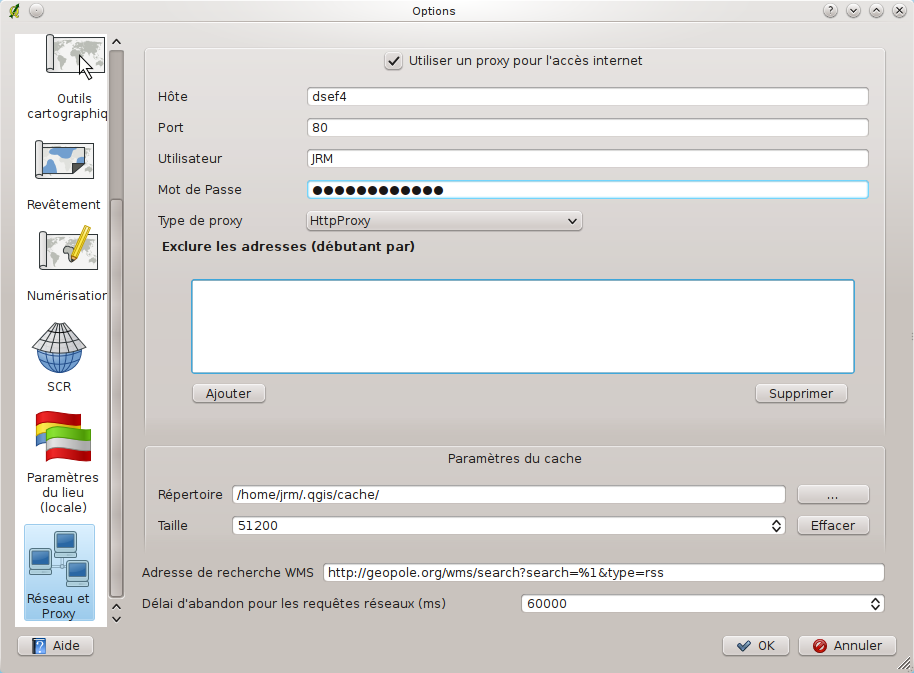
\includegraphics[clip=true, width=14cm]{proxy-settings}
   \caption{Proxy-settings in \qg \nixcaption}
   \label{fig:proxy-settings}
\end{figure}

\begin{Tip} \caption{\textsc{Using Proxies}}
Using proxies can sometimes be tricky. It is useful to 'trial and
error' the above proxy types and check if they succeed in your case.
\end{Tip}

You can modify the options according to your needs. Some of the changes may
require a restart of QGIS before they will be effective.

\begin{itemize}
\item \nix{settings are saved in a texfile: \$HOME/.config/QuantumGIS/qgis.conf}
\item \osx{you can find your settings in: \$HOME/Library/Preferences/org.qgis.qgis.plist}
\item \win{settings are stored in the registry under:}
\begin{verbatim}
\\HKEY\CURRENT_USER\Software\QuantumGIS\qgis
\end{verbatim}
\end{itemize}

\section{Annotation Tools}\label{sec:annotations}
\index{annotations}
\index{text annotation|\see{annotations}}

The 
\includegraphics[width=0.7cm,clip=true]{mActionTextAnnotation} text
annotation tools in the attribute toolbar provides the possibility to
place formated text in a balloon on the QGIS map canvas. Use the text
annotation tool and click into the map canvas.

\begin{figure}[ht]
   \centering
   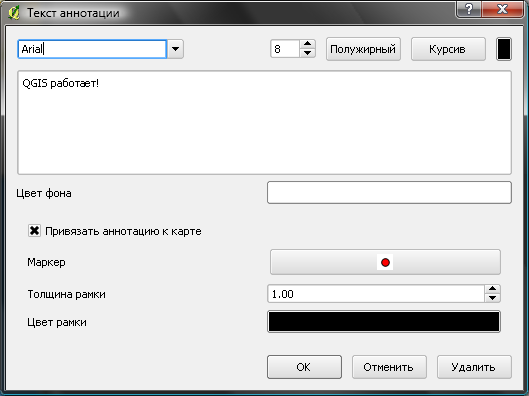
\includegraphics[clip=true, width=12cm]{annotation}
   \caption{Annotation text dialog \nixcaption}
   \label{fig:annotation}
\end{figure}

Double click on the item opens a dialog with various options. There is the
text editor to enter the formated text and other item settings. E.g. there
is the choice of having the item placed on a map position (displayed by
a marker symbol) or to have the item on a screen position (not related
to the map). The item can be moved by map position (drag the map marker)
or by moving only the balloon. The icons are part of gis theme, and are used
by default in the other themes too.

The 
\includegraphics[width=0.7cm,clip=true]{mActionAnnotation} move annotation
tool allows to move the annotation on the map canvas.

\subsection{Form annotations}\index{annotations}
\index{form annotation|\see{annotations}}

Additionally you can also create your own annotation forms. The

\includegraphics[width=0.7cm,clip=true]{mActionFormAnnotation} form annotation
tool is useful to display attributes of a vector layer in a customised qt
designer form (see Figure \ref{fig:custom-annotations}). It is similar to the
designer forms for the identify tool, but displayed in an annotation item.
Also see QGIS blog \url{http://blog.qgis.org/node/143} for more information.

\begin{figure}[ht]
   \centering
   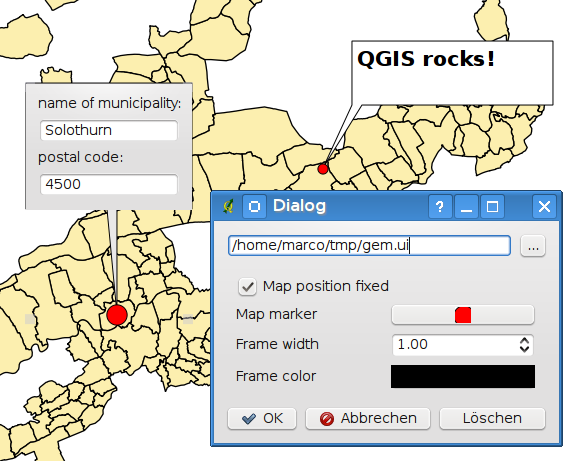
\includegraphics[clip=true, width=10cm]{custom_annotation}
   \caption{Customized qt designer annotation form \nixcaption}
   \label{fig:custom-annotations}
\end{figure}

\textbf{Note:} If you press Ctrl-T while an annotation tool is active 
(move annotation, text annotation, form annotation), the visibility states 
of the items are inverted.

\newpage

\section{Spatial Bookmarks}\label{sec:bookmarks}
\index{bookmarks}
\index{spatial bookmarks|\see{bookmarks}}

Spatial Bookmarks allow you to ``bookmark'' a geographic location and return to it later.

\subsection{Creating a Bookmark}
To create a bookmark:
\begin{enumerate}
\item Zoom or pan to the area of interest.
\item Select the menu option \mainmenuopt{View} \arrow \dropmenuopt{New Bookmark} or press \keystroke{Ctrl-B}.
\item Enter a descriptive name for the bookmark (up to 255 characters).
\item Click \button{OK} to add the bookmark or \button{Cancel} to exit without adding the bookmark.
\end{enumerate}

Note that you can have multiple bookmarks with the same name.

\subsection{Working with Bookmarks}
To use or manage bookmarks, select the menu
option \mainmenuopt{View} \arrow \dropmenuopt{Show Bookmarks}. The \\
\dialog{Geospatial Bookmarks} dialog allows you to zoom to or delete a bookmark.
You can not edit the bookmark name or coordinates.

\subsection{Zooming to a Bookmark}
From the \dialog{Geospatial Bookmarks} dialog, select the desired bookmark by clicking on it,
then click \button{Zoom To}.
You can also zoom to a bookmark by double-clicking on it.

\subsection{Deleting a Bookmark}
To delete a bookmark from the \dialog{Geospatial Bookmarks}
dialog, click on it then click \button{Delete}.
Confirm your choice by clicking \button{Yes} or cancel the
delete by clicking \button{No}.

\section{Live GPS tracking}\label{sec:gpstracking}

To activate Live GPS tracking in QGIS you need to select
\mainmenuopt{View} \arrow \dropmenuopt{Live GPS tracking}. You will get a new
docked Window on the left side of the canvas.

There are 4 possible screens in this GPS tracking window
(see Figure \ref{fig:gpstrack_live} and Figure \ref{fig:gpstrack_options}).

\begin{description}
 \item[(a)] 
\includegraphics[width=0.5cm,clip=true]{mActionToggleEditing}
GPS position coordinates and for manually entering Vertices and Features
 \item[(b)] 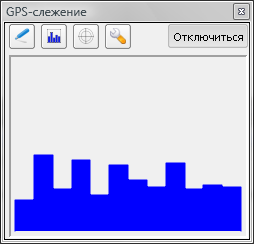
\includegraphics[width=0.5cm,clip=true]{gpstrack_barchart}
GPS signal strength of satellite connections
 \item[(c)] 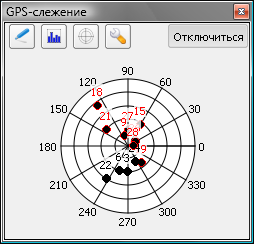
\includegraphics[width=0.5cm,clip=true]{gpstrack_polarchart}
GPS polar screen showing number and polar position of satellites
 \item[(d)] 
\includegraphics[width=0.5cm,clip=true]{mActionOptions}
GPS options screen (see Figure \ref{fig:gpstrack_options}).
\end{description}

With a plugged in GPS receiver (has to be supported by your operating system)
a simple click on \button{Connect} connects the GPS to QGIS. A second click
(now \button{Disconnect} disconnects the GPS-Reciever from you Computer. For 
GNU/Linux gpsd support is integrated to support connection to most GPS 
receivers. Therefore you first have to configure gpsd properly to connect QGIS to it.

[ IMPORTANT ]: If you want to record your position to the canvas you have to
create a new vector layer first and switch it to editable status to be able
to record your track.

\begin{figure}[ht]
\centering
   \subfloat[Position coordinates] {\label{subfig:gpstrack_main}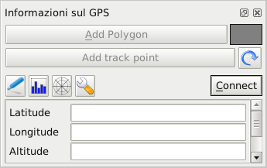
\includegraphics[clip=true, width=0.3\textwidth]{gpstrack_main}}
     \hspace{0.33cm}
   \subfloat[GPS signal strenght]{\label{subfig:gpstrack_stren}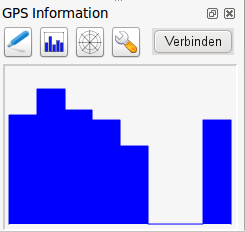
\includegraphics[clip=true, width=0.3\textwidth]{gpstrack_stren}}
     \hspace{0.33cm}
   \subfloat[GPS polar window]{\label{subfig:gpstrack_polar}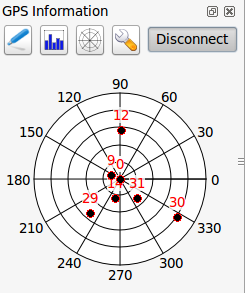
\includegraphics[clip=true, width=0.3\textwidth]{gpstrack_polar}}
\caption{Live GPS tracking \nixcaption} \label{fig:gpstrack_live}
\end{figure}

\begin{figure}[ht]
   \centering
   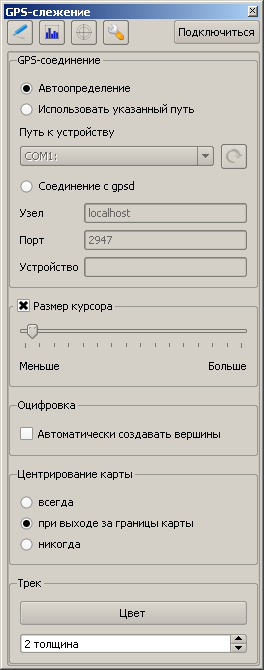
\includegraphics[clip=true, width=4cm]{gpstrack_options}
   \caption{GPS tracking options window \nixcaption}
   \label{fig:gpstrack_options}
\end{figure}

\subsection{Position coordinates}

\includegraphics[width=0.5cm,clip=true]{mActionToggleEditing} If the GPS is
recieving signals from satellites you will see your position in latitude,
longitude and elevation as you can see in Figure \ref{subfig:gpstrack_main}

\subsection{GPS signal strength}
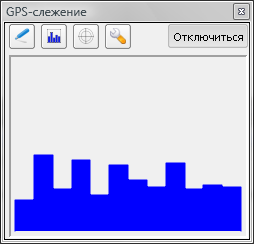
\includegraphics[width=0.5cm,clip=true]{gpstrack_barchart} Here you can see
the signal strenght of the satellites you are revieving signals from
(Figure \ref{subfig:gpstrack_stren}).

\subsection{GPS polar window}
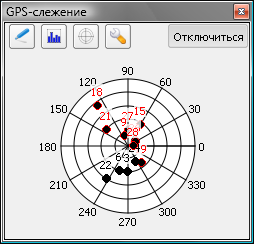
\includegraphics[width=0.5cm,clip=true]{gpstrack_polarchart} If you want
to know where in the sky all the connected satellites are, you have to
switch to the polar screen (Figure \ref{subfig:gpstrack_polar}).
You can also see the ID numbers of the satellites you are recieving signals from.

\subsection{GPS options}

\includegraphics[width=0.5cm,clip=true]{mActionOptions} In case of connection
problems you can switch from \radiobuttonon{Autodetect} to \radiobuttonon{Use
path/port below} and select the path/port your GPS receiver is connected to.
A click on \button{Connect} again initiates the connection to the GPS
receiver.

With the slider \slider{GPS Cursor Size} you can shrink and grow the position
cursor on the canvas. Activating \radiobuttonon{Auto-add vertices} within GPS
digitizing your track will automatically be recorded in the active vector layer
(of course the layer has to be in edit mode).

With GPS map recenter you can decide in which way the canvas will be
updated if your recorded coordinates start either to move out of canvas
or there is any change at all.

Track color and width sets the color of and the width of your drawn track.

If you want to set a feature manually you have to go back to

\includegraphics[width=0.5cm,clip=true]{mActionToggleEditing} ''Position Coordinates''
and click on \button{Add feature}.

\FloatBarrier
